\documentclass{beamer}

\usepackage[utf8]{inputenc}
\usepackage[T1]{fontenc}
\usepackage{graphicx}
\usepackage{hyperref}

\title{Image Embedding for Product Labeling}
\author{Couture Vision}
\date{\today}

\begin{document}

\frame{\titlepage}

\begin{frame}{Sommaire}
\tableofcontents
\end{frame}

\section{Jeu de données}
\begin{frame}{Jeu de données}
\begin{columns}
    \column{0.5\textwidth}
    \begin{figure}
        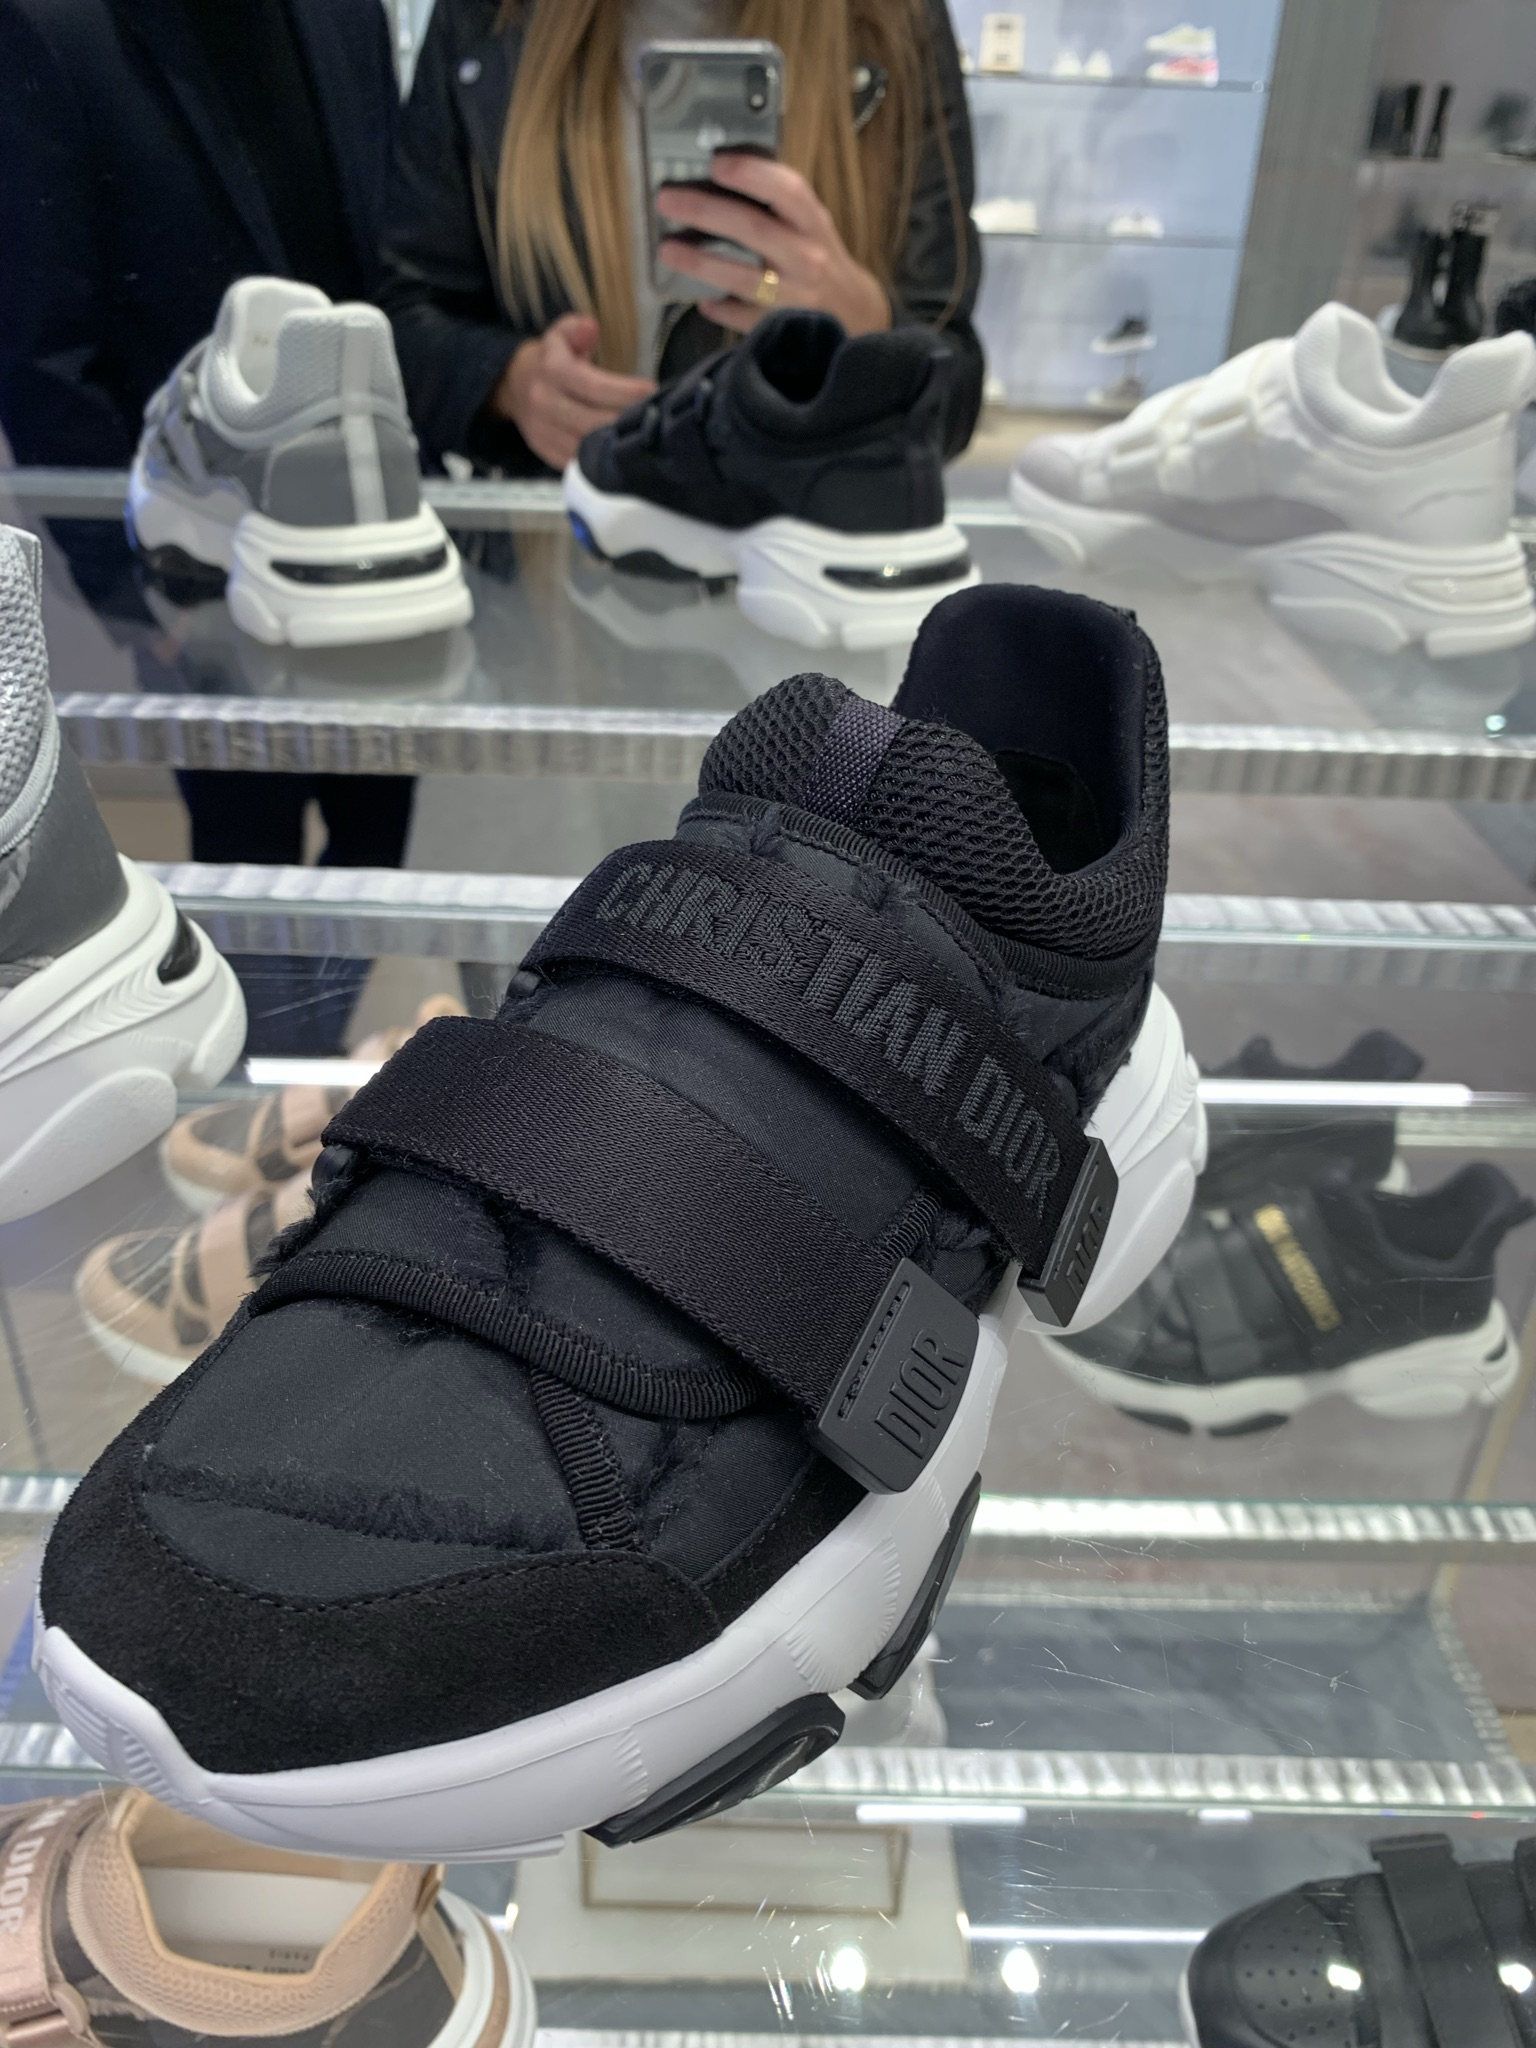
\includegraphics[width=0.6\textwidth]{assets/shoe_test.jpg}
        \caption{Image test}
    \end{figure}
    \column{0.5\textwidth}
    \begin{figure}
        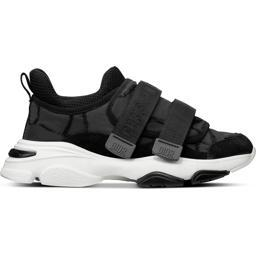
\includegraphics[width=0.6\textwidth]{assets/shoe_reference.jpeg}
        \caption{Image DAM}
    \end{figure}
\end{columns}
\vspace{0.5cm}
\begin{block}{Objectif}
Pour une image test d'article, trouver l'article correspondant dans la base DAM.
\end{block}
\end{frame}

\section{Intuitions}
\begin{frame}{Intuitions}
\begin{itemize}
    \item Utilisation d'un modèle permettant d'extraire l'article de l'image et de mettre un fond blanc derrière.
    \item Utilisation d'un modèle pré-entraîné pour créer des embeddings sur les images DAM et les images de test.
    \item Pour chaque image de test, calcul des similarités cosinus avec tous les embeddings des images DAM et affichage des 5 meilleures similarités (Top-5).
\end{itemize}
\end{frame}

\section{Principe et architecture du modèle retenu}
\begin{frame}{Modèle utilisé}
\begin{itemize}
    \item \textbf{Extraction et traitement de l'article} : Utilisation de \texttt{RMBG} pour rogner l'image et supprimer le fond. 
    \item \textbf{Embeddings d'image} : Modèle ViT par Google (Base Patch-32, 86.4M paramètres).
    \item \textbf{Triplet Network} : Permet d'optimiser les embeddings pour réduire la distance cosinus entre des images similaires.
\end{itemize}
\end{frame}

\section{Amélioration des résultats}
\begin{frame}{Amélioration des résultats}
\begin{itemize}
    \item \textbf{Data augmentation} : Certaines images de test ne sont pas prises du même angle que les images DAM.
    \begin{itemize}
        \item Utilisation de \textbf{TRELLIS} pour générer des modèles 3D.
        \item Exemple :
        \begin{figure}
            \includegraphics[width=0.3\textwidth]{}
            \includegraphics[width=0.3\textwidth]{}
            \includegraphics[width=0.3\textwidth]{}
            \caption{Rendu 3D d'un sac.}
        \end{figure}
    \end{itemize}
    \item Suppression des images de test sans correspondance dans la base DAM.
\end{itemize}
\end{frame}

\section{Evaluation}
\begin{frame}{Evaluation des résultats}
\begin{table}[]
    \centering
    \begin{tabular}{|c|c|c|c|}
    \hline
    \textbf{} & \textbf{Top-1} & \textbf{Top-3} & \textbf{Top-5} \\
    \hline
    Accuracy & 40\% & 60\% & 75\% \\
    \hline
    \end{tabular}
    \caption{Performances du modèle.}
\end{table}
\end{frame}

\section{Expérimentations non concluantes}
\begin{frame}{Expérimentations non concluantes}
\begin{itemize}
    \item \textbf{Amélioration du Top-1 par NLP} :
    \begin{itemize}
        \item Utilisation du modèle BLIP pour générer des descriptions d'articles.
        \item Objectif : éviter les erreurs de couleur ou de texture.
        \item Limite : Les descriptions générées sont trop pauvres pour améliorer significativement les résultats.
    \end{itemize}
\end{itemize}
\end{frame}

\section{Conclusion}
\begin{frame}{Conclusion}
\begin{itemize}
    \item Modèle performant grâce à l'ajout de rendus 3D et la combinaison des embeddings 2D/3D.
    \item Résultats encourageants avec une précision Top-1 de 40\%, mais améliorable.
    \item Pistes futures :
    \begin{itemize}
        \item Utilisation de modèles NLP avec plus de paramètres pour enrichir les descriptions d'images.
    \end{itemize}
\end{itemize}
\end{frame}

\end{document}
